\section{Metropolis Hasting for Bayesian Inference using FFBS  within the Gibbs Sampling On MJPs}~

\setlength{\unitlength}{0.8cm}
  \begin{figure}[H]
  \centering
  \begin{minipage}[!hp]{0.45\linewidth}
  \centering
    \includegraphics [width=0.70\textwidth, angle=0]{figs/plotn0.pdf}
      \end{minipage}
  \begin{minipage}[!hp]{0.45\linewidth}
  \centering
    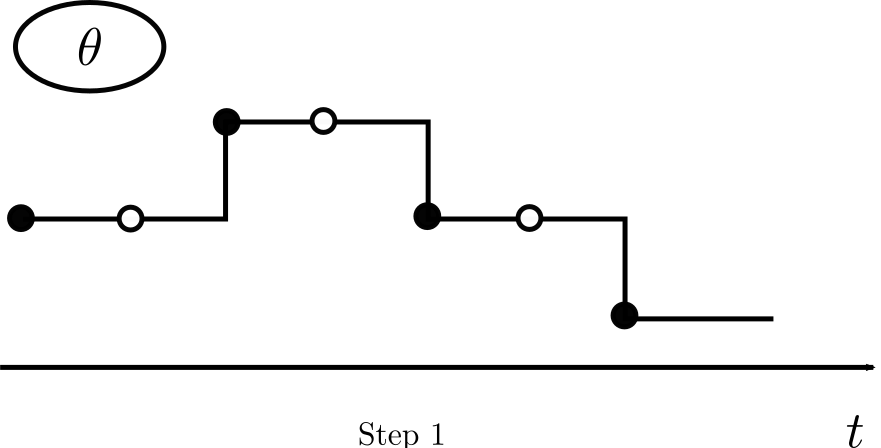
\includegraphics [width=0.70\textwidth, angle=0]{figs/plotn1.pdf}
    \vspace{-0 in}
  \end{minipage}
  \begin{minipage}[!hp]{0.45\linewidth}
  \centering
    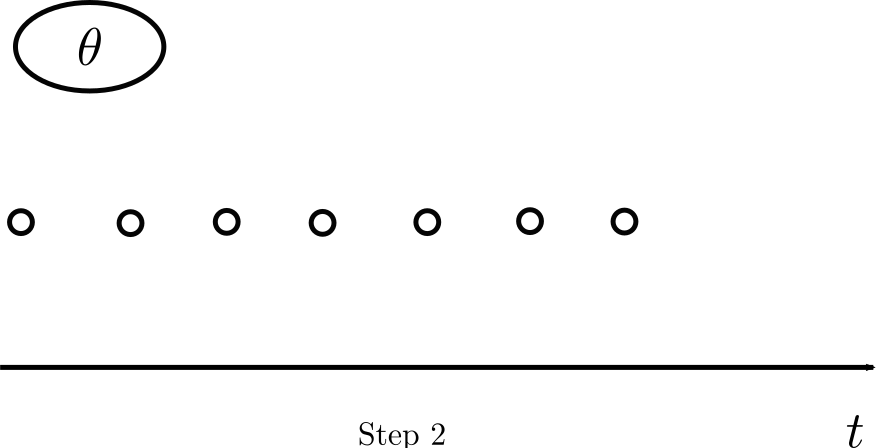
\includegraphics [width=0.70\textwidth, angle=0]{figs/plotn2.pdf}
    \vspace{-0 in}
  \end{minipage}
  \begin{minipage}[!hp]{0.45\linewidth}
  \centering
    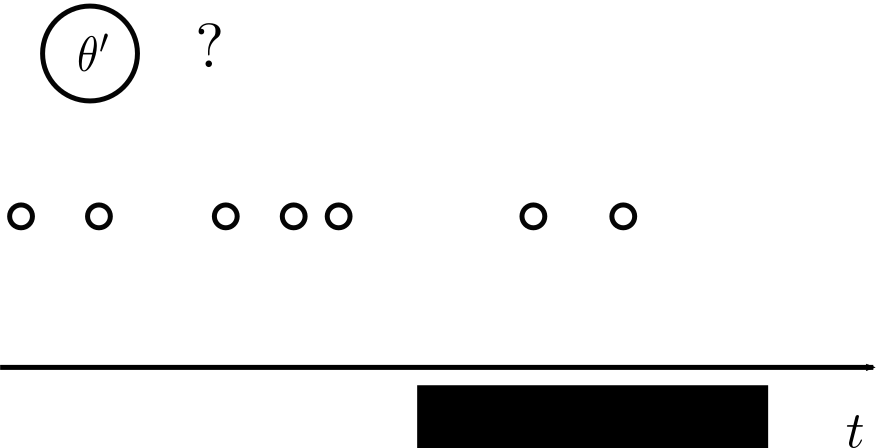
\includegraphics [width=0.70\textwidth, angle=0]{figs/plotn3.pdf}
    \vspace{-0 in}
  \end{minipage}
  \begin{minipage}[!hp]{0.45\linewidth}
  \centering
    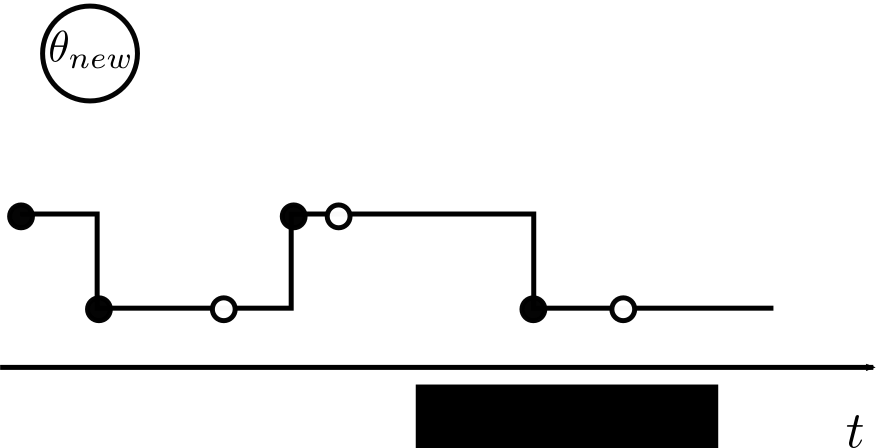
\includegraphics [width=0.70\textwidth, angle=0]{figs/plotn4.pdf}
    \vspace{-0 in}
  \end{minipage}
  \begin{minipage}[!hp]{0.45\linewidth}
  \centering
    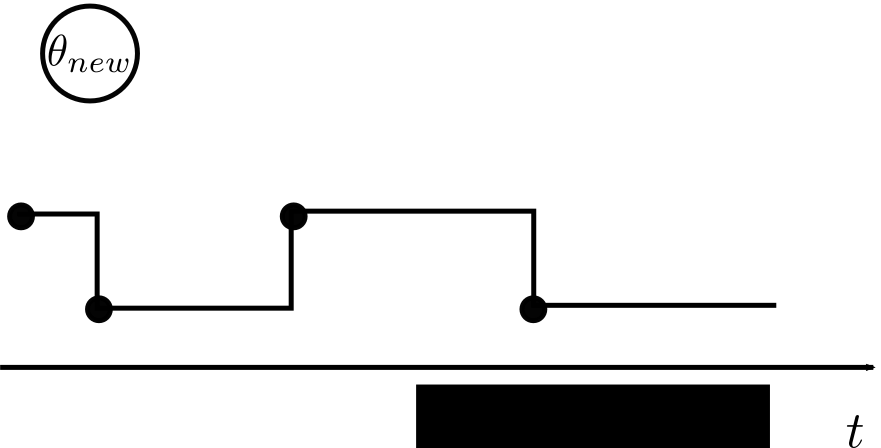
\includegraphics [width=0.70\textwidth, angle=0]{figs/plotn5.pdf}
    \vspace{-0 in}
  \end{minipage}
  \caption{\Naive\ MH-algorithm. Step 0 to 2: sample thinned events
  and discard state information to get a random grid. Step 3: 
propose a new parameter $\theta'$, and accept or reject by making
a forward pass on the grid. Steps 4 to 5: make a backward pass using
the accepted parameter and discard self-transitions to produce a new
trajectory.}
   \label{fig:naive_mh}

  \end{figure}

\begin{algorithm}[H]
   \caption{MH In Gibbs sampling for MJPs }
   \label{alg:MH In Gibbs}
\begin{algorithmic}
  \State 
  \begin{tabular}{l l}
   \textbf{Input:  } & \text{A set of partial and noisy observations $y_{[t_0, t_{N+1})}$}, \\
                      & \text{Initial distribution over states $\pi_0$,  Metropolis Hasting proposal $q(. | \theta)$}.\\
                      & \text{The previous MJP path $S(t) = (S, T)$, the previous MJP parameters $\theta$}.\\ 
 \textbf{Output:  }& \text{A new MJP trajectory $\tilde{S} (t) = (\tilde{S}, \tilde{T})$, A series of MJP parameters $\tilde{\theta}$}.
   \end{tabular}
   \hrule \\
    \State 1: Let $\Omega = h(\theta)$, with $\Omega > \max_s{|A_s|}$ using some deterministic function $h$.
    \State 2: Sample virtual jumps $U\subset[t_{start}, t_{end}]$ from a Non homogeneous Poisson process with piecewise-constant rate$$R(t) = (\Omega + A_{S(t)}).$$\\Define $W = T \cup U$.
    \State 3: Propose $\theta^* \sim q(.| \theta)$.\\
        Accept $\theta^*$ as $\tilde{\theta}$ with probability $\alpha$.
        \begin{align*}
        \alpha &=  1 \wedge \frac{P(W,\theta^*| y)}{P(W, \theta| y)} \frac{q(\theta|\theta^*)}{q(\theta^*|\theta)}\\
        &=  1 \wedge \frac{P(y| W,\theta^*) P(W | \theta^*)p(\theta^*)}{P(y|W, \theta)P(W | \theta)p(\theta)} \frac{q(\theta|\theta^*)}{q(\theta^*|\theta)}.
        \end{align*}
    \State 4: Sample a path $\tilde{V}$, from a discret-time Markov chain with $|W| + 1$ steps, using FFBS algorithm. The transition matrix of the Markov chain is $B = (I + \frac{A}{\Omega})$ while the initial distribution over states is $\pi_0$. The likelihood of state $s$ at step $i$ is 
    $$ L_i(s) = P(Y_{[w_i, w_{i + 1})} | S(t) = s \; for\; t \in [w_i, w_{i + 1})) = \prod_{j: t_j \in [w_i, w_{i + 1})}p(y_{t_j} | S(t_j) = s).$$\\
%(i.e. $V(i) \sim P(V |  \theta(i), W(i - 1), y).$) Then delete all the virtual jumps to get $S(i), T(i) .$\\
    \State 5: Let $\tilde{T}$ be the set of times in $W$ when the Markov chain changes state. Define $\tilde{S}$ as the corresponding set of state values. Return $(\tilde{S}, \tilde{T}, \tilde{\theta})$.\\
\end{algorithmic}
\end{algorithm}
\label{sec:meth}

The key idea of the dependent-thinning approach of~\cite{RaoTeh13} is
to introduce the set of thinned candidate transition times. These,
along with the extant transition times, form a random grid,
conditioned on which sampling a new trajectory reduces to a 
standard discrete-time HMM sampling step. This suggests incorporating
the MH-step outlined earlier to update the parameters $\theta$
with the trajectory integrated out, but now conditioned on the random
grid. Figure~\ref{fig:naive_mh} outlines this idea.
An iteration begins with a current parameter $\theta$ and a current
trajectory $S(t)$. As with~\cite{RaoTeh12}, we first sample
a new set of thinned events from a Poisson process with rate
$B_{S(t)}-A_{S(t)}$. This, along with the transition times of
$S(t)$ form a new random grid. Now, we propose a new parameter 
$\theta'$ from some proposal distribution $q(\theta'|\theta)$,
and make a forward pass over the grid, to calculate the marginal
probabilities $p(X|W,\theta$ and $p(X|W,\theta')$. These can be
used to calculate the MH-acceptance probability, and after accepting
or rejecting $\theta'$, a new parameter can be sampled by making
a backward pass through $W$.

It is important to note however that the parameter $\theta$
determines not just the MJP trajectory $S(t)$, and with $S(t)$ 
marginalized out, the observations $X$. The random grid $W$ itself
is distributed differently for different values of $\theta$. For
the simple uniformization approach of~\cite{RaoTeh13}, $W$ is
distributed as a homogeneous Poisson process with rate $\Omega = 
2 \max A(\theta)$, while under the more general scheme of~\cite{RaoTeh12},
it follows a state-dependent generative scheme who probability can
never-the-less be calculated easily during the forward pass.
Thus, the MH MH-acceptance probability is given by $\min(1,
  \frac{p(\theta,X,W}{p(\theta',X,W)}$. Thus the acceptance probability
involves two terms: how compatible the new parameter $\theta'$ is
with the observations, and how compatible it is with the random
grid $W$. The first effect is inevitable, however in our experiments,
we found the second also has a significate effect of the MH-acceptance
probability. In the next section, we describe a way around this
issue. 
